\documentclass[11pt]{article}
\usepackage{icmlko}
\begin{document}

\title{위약을 어디서 섞느냐가 무엇을 검사하는지 정한다 --- 내 '눈금' 설명이 틀렸다}
\author{월드모델 실험실}
\date{노트 392 · 2026년 8월 1일}
\maketitle

\begin{abstract}
노트 391이 펀딩의 새 학습 행을 기존 라벨 범위 \emph{안}과 \emph{밖}으로
갈라, 안은 위약이 이득을 지우고(잔량 $-23$\%) 밖은 못 지운다(104\%)는 것을
보였다. 그리고 설명을 붙였다 --- \emph{안의 행은 정보를 주고 밖의 행은
눈금을 준다.}

\textbf{그 설명은 스스로 모순이다.} 스피어만은 예측의 단조 변환에 불변이라
``눈금''이 순위 상관을 움직일 수 없다. 그래서 시험했다.

위약을 하나 더 만들었다. \textbf{위약1}은 새 행끼리 라벨을 섞는다(노트
389 · 391이 쓴 것). \textbf{위약2}는 새 행의 라벨을 \emph{옛 학습 행의
라벨과 맞바꾼다} --- 낮은 축을 가진 새 행에 높은 라벨이 가고 그 반대도
간다. 사전 등록: \emph{눈금 설명이 맞다면 위약2도 이득을 못 지운다}(라벨
분포는 그대로이므로).

\begin{center}
\begin{tabular}{lrrl}
\hline
팔 & 펀딩 차 & 부호 & 잔량 \\
\hline
D 실제 (밖 326행) & $+0.1091$ & 12/12 & --- \\
E 위약1 (새끼리 섞기) & $+0.1142$ & 12/12 & 105\% \\
F \textbf{위약2} (옛 것과 맞바꿈) & $\mathbf{-0.2136}$ & \textbf{0/12} & $\mathbf{-196\%}$ \\
\hline
\end{tabular}
\end{center}

\textbf{위약2가 이득을 지우는 정도가 아니라 뒤집는다.} 눈금 설명은
반증됐다. \textbf{밖의 행이 나르는 것은 무리 수준 연합이다} --- ``이런
축을 가진 것들은 라벨이 낮다.'' 새 것끼리 섞어도 그 연합은 그대로 남고,
옛 것과 맞바꾸면 연합이 \emph{거꾸로} 실려 예측이 반대로 간다.

\textbf{그래서 조항 ⑤를 다시 고친다.} 위약을 어디서 섞느냐가 무엇을
검사하는지 정한다 --- 범위 \emph{안}의 행은 새 것끼리 섞기가 옳은 위약이고
(그 행들이 나르는 것이 행 수준 짝이므로), 범위 \emph{밖}의 행은 새 것끼리
섞기가 \textbf{아무것도 검사하지 않는다}. 옛 것과 맞바꿔야 한다.

그리고 노트 391의 결론을 정정한다: 노트 381 이득의 46\%는 \emph{정보가
아닌 것}이 아니라 \textbf{무리 수준 정보}였다.
\end{abstract}

\section{왜 내 설명을 의심했나}

노트 391은 밖의 326행이 위약을 통과하지 못하는 것을 보고 ``눈금을 준다''고
적었다. 하루 뒤에 읽으니 앞뒤가 안 맞는다 --- \textbf{판정치가 스피어만
순위 상관이다.} 예측에 상수를 더하거나 곱해도 순위가 안 변하니 값이
안 변한다. ``눈금이 옮겨 가서 점수가 올랐다''는 문장은 이 판정치에서
성립할 수 없다.

그러면 위약1을 통과하고도 남는 그것은 무엇인가. 위약1이 지우는 것은
\emph{어느 새 행에 어느 새 라벨이 붙었나}뿐이다. 안 지워지는 것이 둘
있다 --- 새 행들의 \emph{축 분포}와 그 행들의 \emph{라벨 다발}. 둘이
같이 남으면 ``이 축 영역은 라벨이 낮다''가 남는다. \textbf{그것은 눈금이
아니라 연합이고, 세상에 대한 참일 수도 있다.}

\section{위약2}

가르는 방법은 그 연합을 깨는 것이다. 새 행 326개의 라벨을 옛 학습
320행의 라벨과 \textbf{맞바꾼다}(짝 320개, 씨앗 고정). 그러면

\begin{itemize}
\item 학습 전체의 라벨 다발은 \textbf{그대로}다 --- 눈금 설명이 예측하는
효과는 유지된다.
\item 새 행(낮은 축 영역)에 옛 행의 \emph{높은} 라벨이 붙고, 옛 행에 새
행의 \emph{낮은} 라벨이 붙는다 --- 무리 수준 연합이 \textbf{거꾸로}
실린다.
\end{itemize}

\textbf{사전 등록:} 눈금이면 위약2도 이득을 못 지운다. 연합이면 위약2가
이득을 지우고, 거꾸로 실렸으니 아마 음수로 간다.

\begin{figure}[t]
\centering
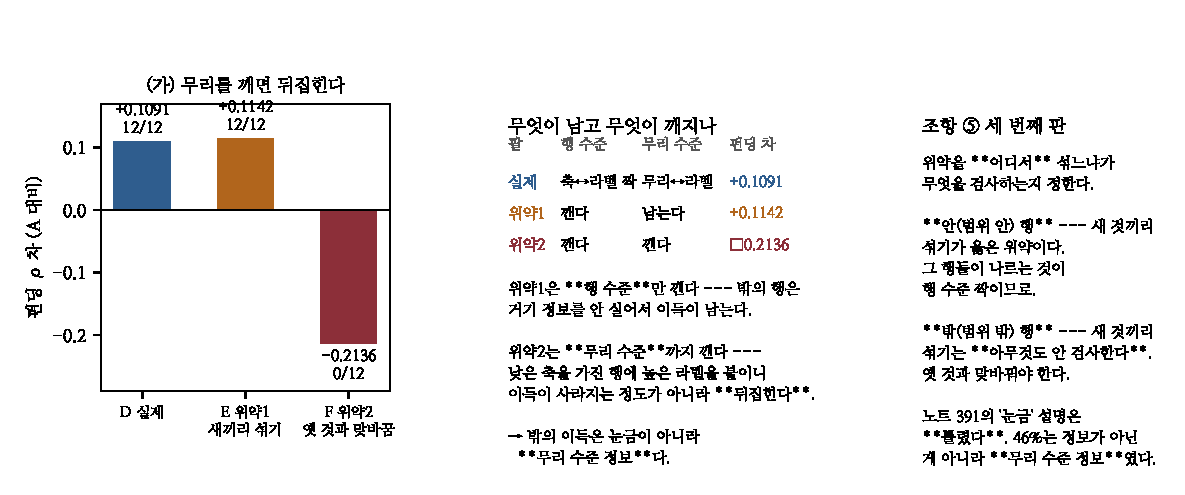
\includegraphics[width=\linewidth]{figs/fig392.pdf}
\caption{\textbf{(가)} 세 팔. 위약1은 이득을 그대로 내고 위약2는 뒤집는다.
\textbf{(나)} 각 위약이 무엇을 깨는지. \textbf{(다)} 조항 ⑤의 세 번째 판.}
\label{fig:main}
\end{figure}

\section{결과 --- 뒤집힌다}

$-0.2136$ · \textbf{0/12}. A(아무것도 안 넣은 팔)보다 한참 아래다. 실제
팔이 $+0.1091$ 이었으니 위약2는 그 이득을 지우고도 $0.32$ 를 더 깎았다.

\textbf{눈금 설명은 반증됐다.} 라벨 다발이 그대로인데 이득이 뒤집혔으므로,
남아 있던 것은 분포가 아니라 \emph{어느 축 영역이 어느 라벨과 가는가}였다.
위약1은 그 연합을 안 건드리므로 105\%가 남았고, 위약2는 그것을 거꾸로
실어서 음수가 됐다.

\textbf{그러니 밖의 326행은 진짜 정보를 나른다.} 다만 그 정보가 행 하나
하나가 아니라 무리에 실려 있다. 노트 391이 ``이득의 46\%는 정보가
아니었다''고 쓴 것을 정정한다 --- \textbf{46\%는 무리 수준 정보였다.}

\section{조항 ⑤ --- 세 번째 판}

노트 389가 만들고 노트 391이 한 번 고친 조항을 다시 고친다.

\begin{center}
\begin{tabular}{lll}
\hline
더하는 행 & 옳은 위약 & 무엇을 검사하나 \\
\hline
기존 범위 \textbf{안} & 새 것끼리 섞기 & 행 수준 짝(축$\leftrightarrow$라벨) \\
기존 범위 \textbf{밖} & \textbf{옛 것과 맞바꾸기} & 무리 수준 연합 \\
\hline
\end{tabular}
\end{center}

\textbf{범위 밖 행에 새 것끼리 섞기를 쓰면 아무것도 검사하지 않는다} ---
그 행들이 나르는 정보가 그 위약이 안 건드리는 자리에 있기 때문이다. 노트
389가 만화를 기각한 근거가 바로 그 위약이었으니, \textbf{만화도 다시
봐야 한다}(만화의 4,999행은 100\% 밖이었다).

\textbf{규약 문장:} 학습 행을 더해 이득을 주장할 때는 위약이 그 이득을
지워야 한다. \emph{위약은 더하는 행이 기존 범위 안이면 새 것끼리 섞고,
밖이면 옛 학습 행과 맞바꾼다.} 섞여 있으면 갈라서 각각 맞는 위약을 쓴다.

\section{남은 것}

\begin{center}
\begin{tabular}{lll}
\hline
항목 & 왜 값이 큰가 & 어떻게 \\
\hline
만화 4,999 다시 & 노트 389가 틀린 위약으로 기각했다 & 위약2로 다시 \\
웹툰 835 안/밖 분해 & 아직 안 갈랐다 & 다섯 팔 설계 \\
애니 아카이브 & 무게 606 · 덮음 22\% & 수집 중 \\
무리 수준 정보를 판이 세나 & 판정치가 그것을 다 못 볼 수 있다 & 무리 표시자로 상한을 잰다 \\
\hline
\end{tabular}
\end{center}

\end{document}
